\documentclass[xcolor=dvipsnames]{beamer}
\usetheme{metropolis}      
\definecolor{UniBlue}{RGB}{255,255,255}

\setbeamercolor{frametitle}{fg=Brown,bg=Gray!10}
\setbeamercolor{section in head/foot}{bg=Brown}
\setbeamercolor{author in head/foot}{bg=Brown}
\setbeamercolor{date in head/foot}{fg=Brown}
\addtobeamertemplate{frametitle}{}{\vspace{-10em}} % increase

\setbeamertemplate{frametitle}{%
	\usebeamerfont{frametitle}\insertframetitle\strut%
	\vskip0.8\baselineskip%
	\leaders\vrule width \paperwidth\vskip0.5pt%
	\vskip0pt%
	\nointerlineskip
}

\usepackage{tikz}
\usepackage[utf8]{inputenc}

\usepackage{pgfplots}
\pgfplotsset{compat=newest}


     % Use metropolis theme
\title{Gaussian Processes}
\date{\today}
\author{Nipun Batra}
\institute{Machine Learning CS 612}
\begin{document}
  \maketitle
  \section{First Section}
  \begin{frame}{First Frame}
    Hello, world!
  \end{frame}
  \begin{frame}{First Frame}
Hello, world!
\end{frame}
  \begin{frame}{First Frame}
Hello, world!
\end{frame}

\section{Section2}
  \begin{frame}{First Frame}
  \begin{itemize}
  	\item Hello, world!
\begin{figure}
	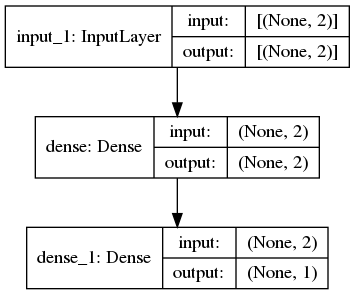
\includegraphics[scale=0.3]{../notebooks/model}
	\caption{Figure 1}
	\label{fig:model}
\end{figure}
  \end{itemize}

\end{frame}
\begin{frame}



%
\end{frame}
\end{document}